%
% qq.tex
%
% (c) 2021 Prof Dr Andreas Müller, OST Ostschweizer Fachhochschule
%
\documentclass[tikz]{standalone}
\usepackage{times}
\usepackage{amsmath}
\usepackage{txfonts}
\usepackage[utf8]{inputenc}
\usepackage{graphics}
\usetikzlibrary{arrows,intersections,math}
\usepackage{ifthen}
\begin{document}

\definecolor{darkred}{rgb}{0.7,0,0}

\newboolean{showgrid}
\setboolean{showgrid}{false}
\def\breite{4}
\def\hoehe{4}

\begin{tikzpicture}[>=latex,thick]

% Povray Bild
\begin{scope}[xshift=-3.3cm]
\node at (0,0) {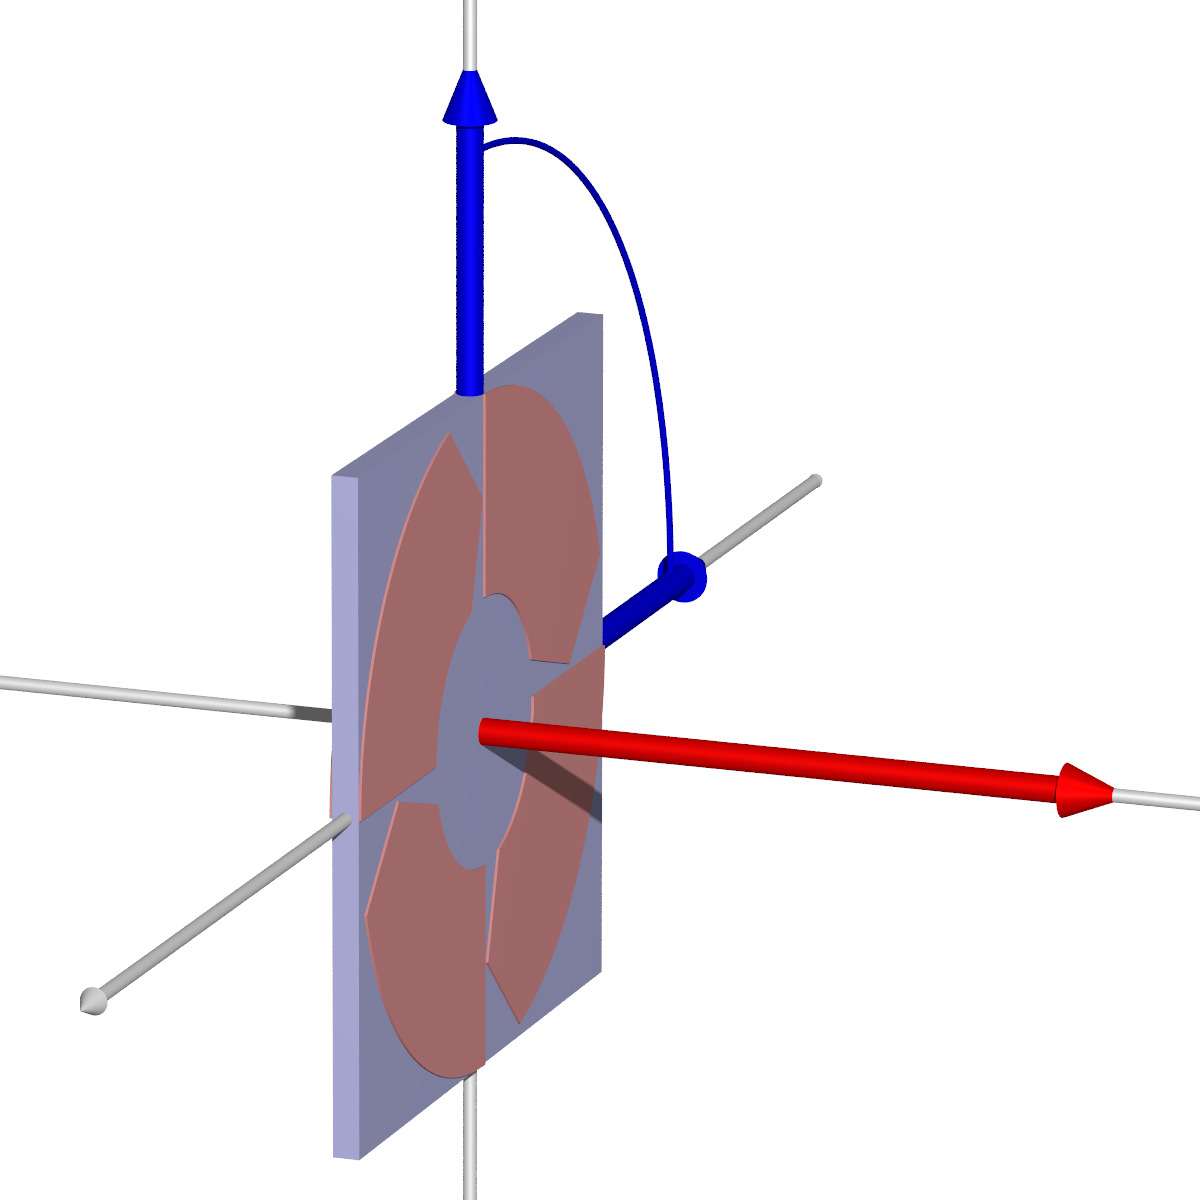
\includegraphics[width=6.3cm]{q23.jpg}};
% Gitter
\ifthenelse{\boolean{showgrid}}{
\draw[step=0.1,line width=0.1pt] (-\breite,-\hoehe) grid (\breite, \hoehe);
\draw[step=0.5,line width=0.4pt] (-\breite,-\hoehe) grid (\breite, \hoehe);
\draw                            (-\breite,-\hoehe) grid (\breite, \hoehe);
\fill (0,0) circle[radius=0.05];
}{}
\fill[color=white,opacity=0.5] ({-0.6-0.3},{-0.2-0.2}) rectangle ({-0.6+0.3},{-0.2+0.2});
\node[color=darkred] at (-0.6,-0.2) {$q_{23}$};
\node[color=blue] at (-0.4,2.7) {$\mathbf{v}$};
\node[color=blue] at (0.7,0.4) {$\mathbf{v}''_{23}$};
\node at (3.1,-1.4) {$a_1$};
\node at (-2.7,-2.4) {$a_3$};
\node at (-0.7,3.4) {$a_2$};
\end{scope}

\setboolean{showgrid}{false}

\begin{scope}[xshift=3.3cm]
\node at (0,0) {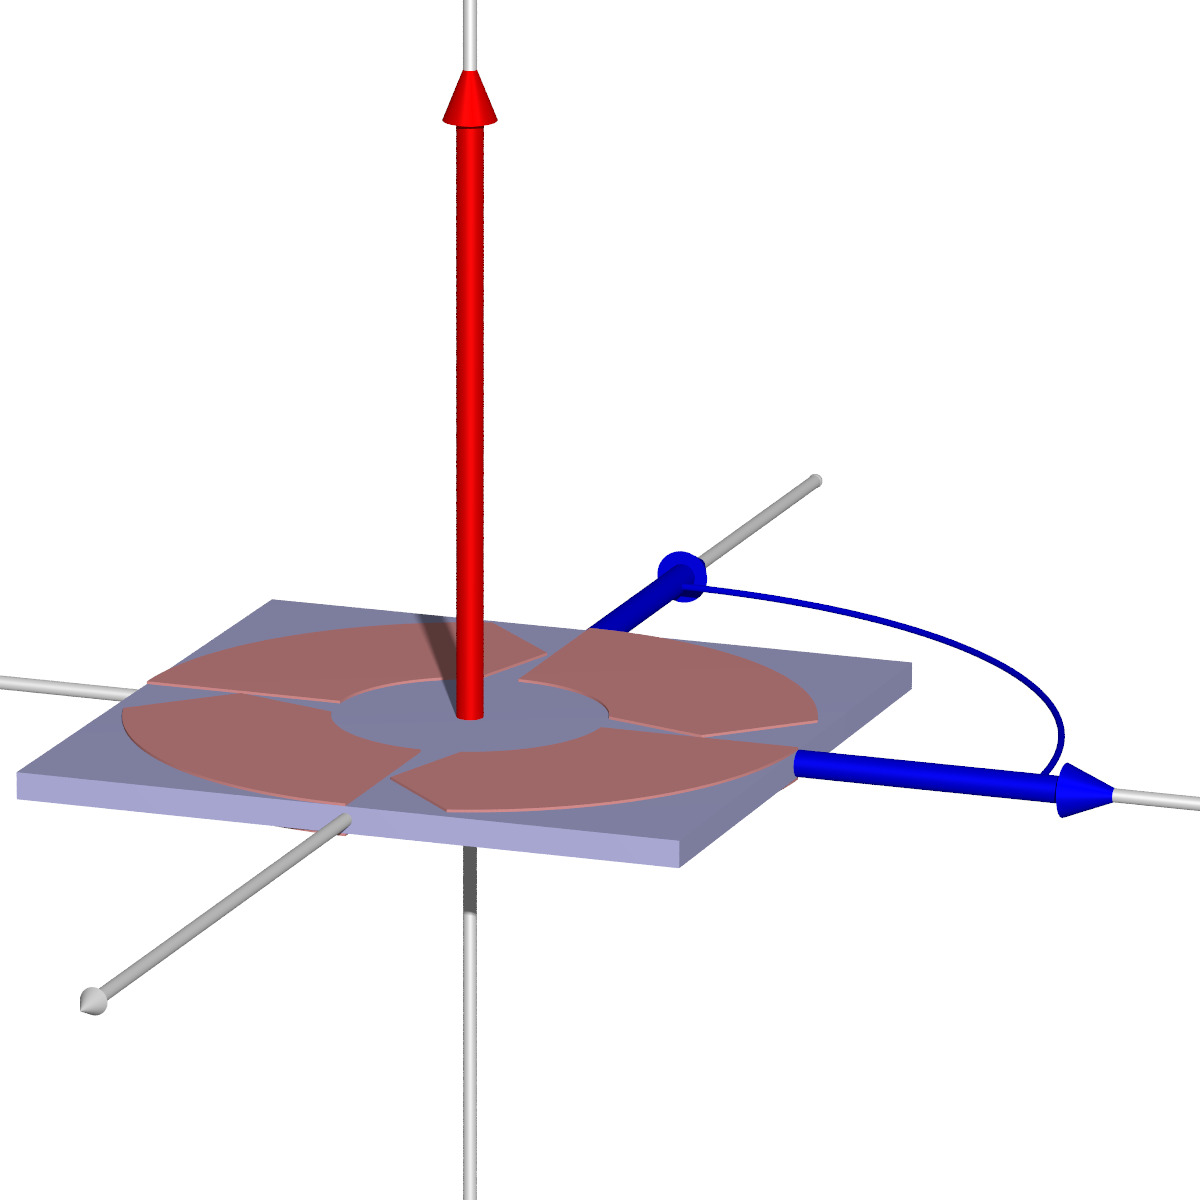
\includegraphics[width=6.3cm]{q31.jpg}};
% Gitter
\ifthenelse{\boolean{showgrid}}{
\draw[step=0.1,line width=0.1pt] (-\breite,-\hoehe) grid (\breite, \hoehe);
\draw[step=0.5,line width=0.4pt] (-\breite,-\hoehe) grid (\breite, \hoehe);
\draw                            (-\breite,-\hoehe) grid (\breite, \hoehe);
\fill (0,0) circle[radius=0.05];
}{}
\fill[color=white,opacity=0.5] ({-0.7-0.3},{-0.9-0.2}) rectangle ({-0.7+0.3},{-0.9+0.2});
\node[color=darkred] at (-0.7,-0.9) {$q_{13}$};
\node[color=blue] at (0.7,0.4) {$\mathbf{v}''_{23}$};
\node[color=blue] at (2.7,-0.7) {$\mathbf{v}''$};
\node at (3.1,-1.4) {$a_1$};
\node at (-2.7,-2.4) {$a_3$};
\node at (-0.7,3.4) {$a_2$};
\end{scope}


\end{tikzpicture}

\end{document}

